\chapter{Estratégias de RVD/B}
\label{sec:Estrategias_RVDB}

% Neste capítulo descreve-se as estratégias empregadas para o processo de RVD/B entre o veículo visitante e o alvo. O objetivo é aplicar o modelo dinâmico e as leis de controle desenvolvidas no Capítulo 2 a um cenário de missão, considerando as diferentes fases de aproximação e os requisitos operacionais associados.
% Inicialmente, apresentam-se as fases da sequência de aproximação, desde a injeção orbital até o momento da captura. Depois, são definidos os corredores de aproximação, as zonas de segurança e os critérios de transição entre as etapas.
% O capítulo aborda o perfil de atitude do \textit{chaser}, a integração entre guiagem e controle e os requisitos de navegação.
% Por fim, as métricas de desempenho são apresentadas e os critérios de sucesso utilizados para avaliar a efetividade da estratégia de aproximação adotada.

% \section{Objetivo e escopo}
\label{sec:objetivo_escopo}

As estratégias descritas nesta seção estabelece a sequência lógica de aproximação entre o veículo visitante e o alvo.
Neste capítulo a análise concentra-se nas fases operacionais, na definição dos corredores de aproximação, nos limites de segurança e nos critérios que determinam as transições entre as etapas.
A estrutura geral segue a abordagem apresentada por
\cite{fehse2003}, complementada por princípios de controle e modelagem orbital discutidos por \cite{alfriend2010}.
Dessa forma, o capítulo abrange a descrição das fases de aproximação, o comportamento da espaçonave visitante, os requisitos de navegação e a integração entre os módulos de guiagem e controle.
% \section{Fases da missão de RVD/B}
\label{sec:fases_operacionais}

A sequência operacional foi dividida em fases, que se estendem desde a injeção orbital até o instante de captura.

\subsection{Injeção orbital inicial}

Após o lançamento, o veículo lançador insere o veículo visitante em uma órbita circular.
Nesse instante, o argumento de latitude do visitante do alvo são diferentes, por outro lado, os outros elementos orbitais de ambas as espaçonaves, como a excentricidade, inclinação, longitude do nodo ascendente e argumento do perigeu, são iguais.
Portanto, as diferenças iniciais entre o veículo visitante e o alvo se dão pelo argumento de latitude e por suas altitudes.

\begin{figure}[ht]
    \label{fig:injecao_orbita_inicial}
\centering
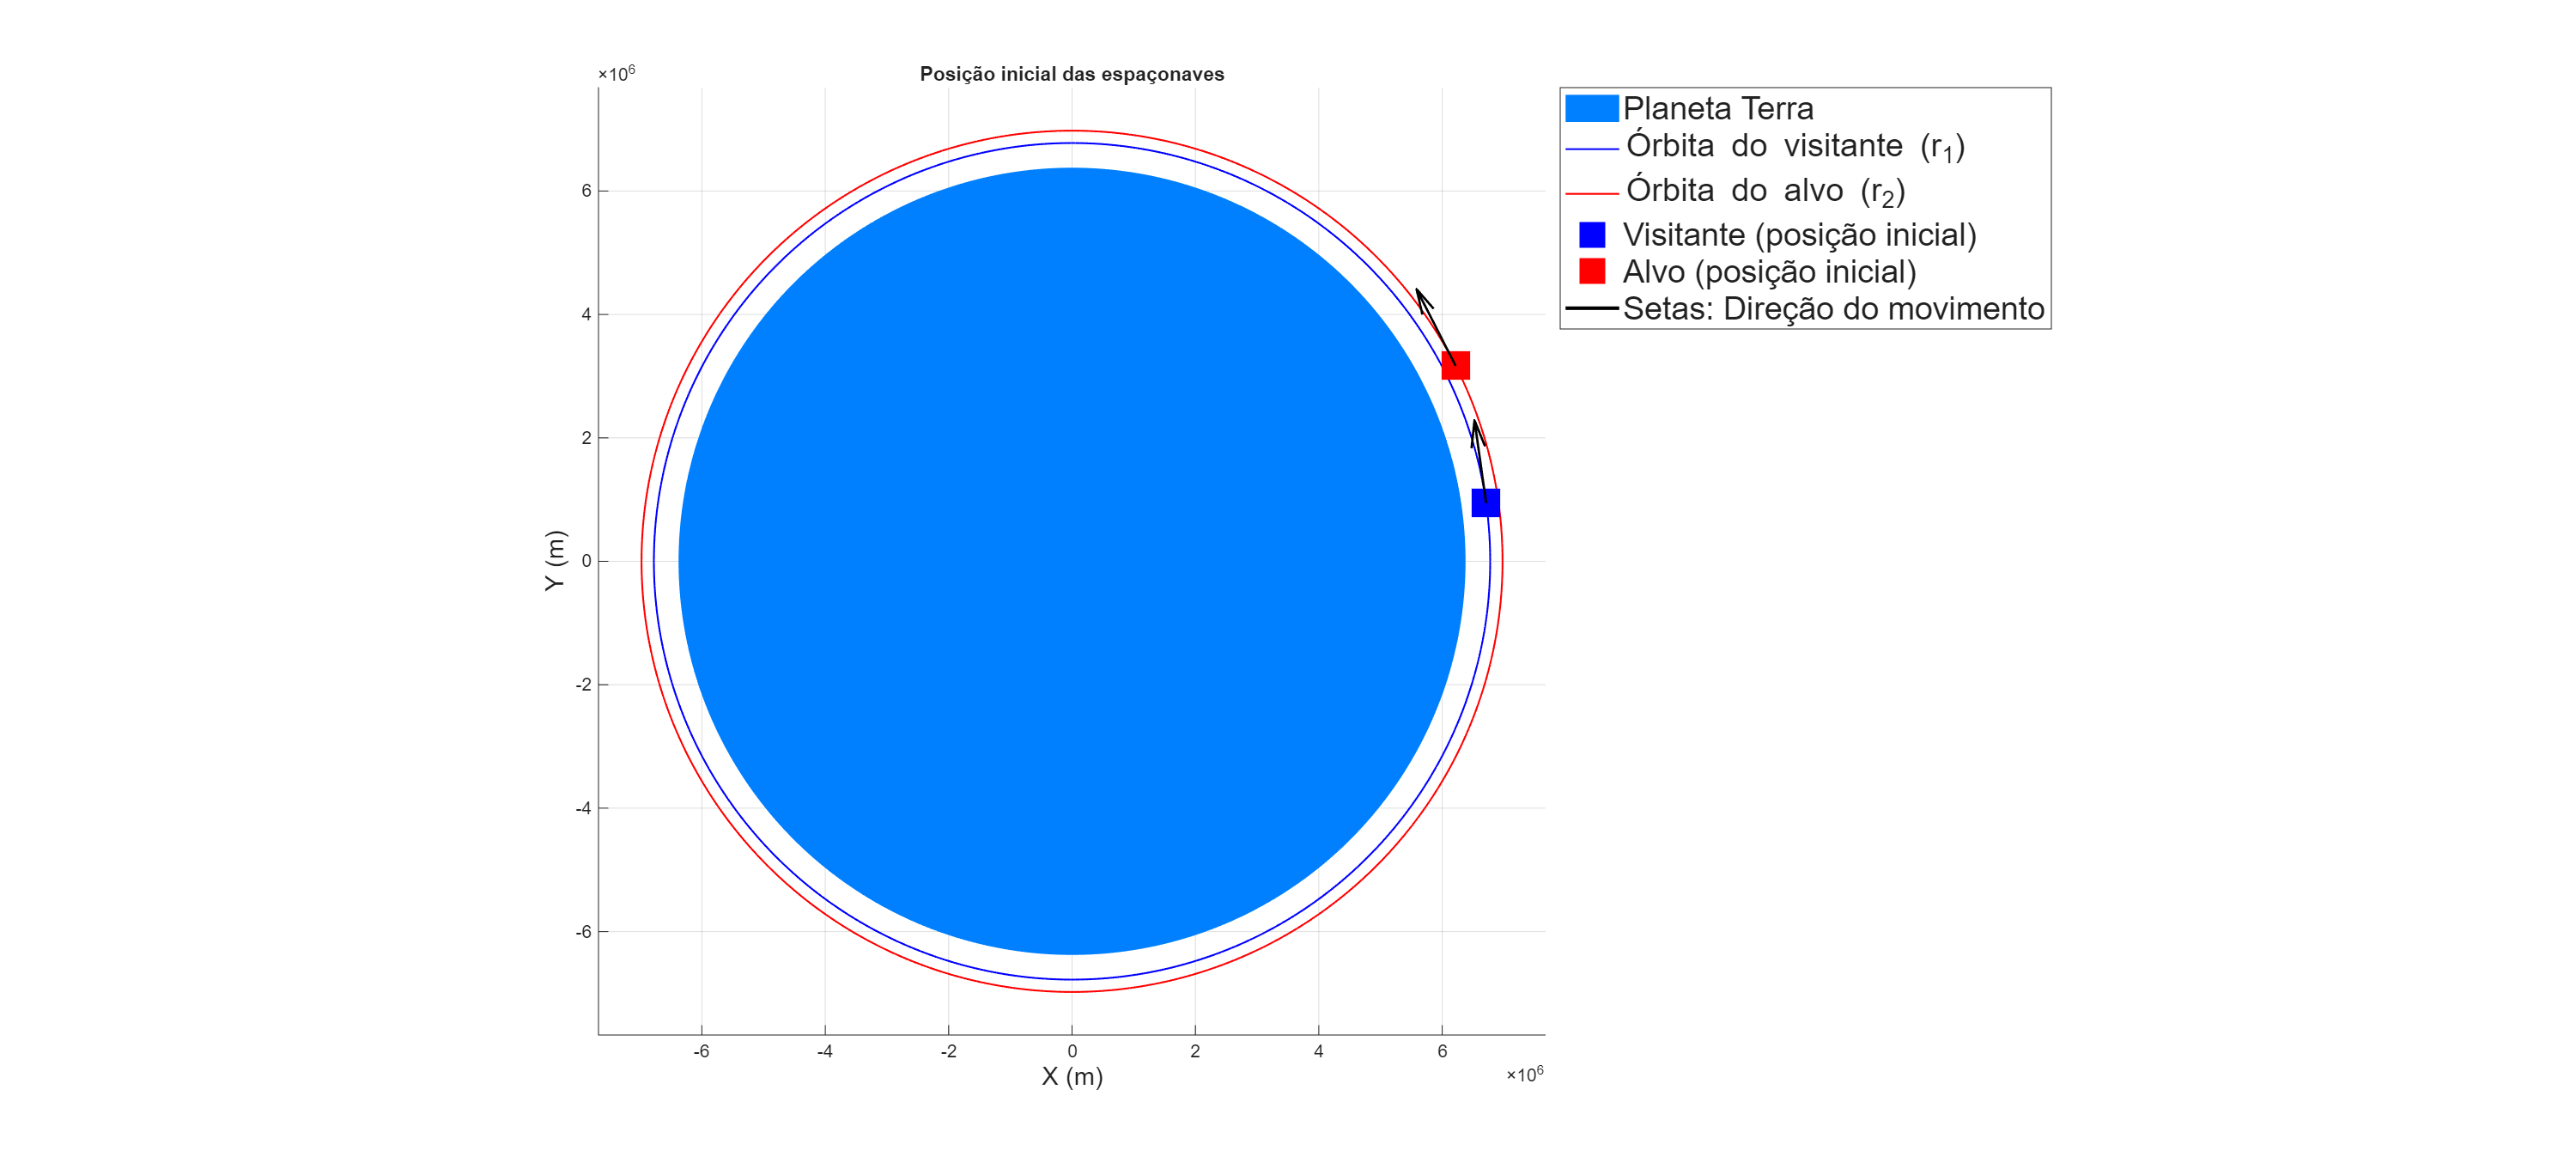
\includegraphics[width=1\linewidth]{3 Estrategia de RVDB/Imagens/1 Injecao orbita inicial.png}
\caption{Posição inicial das espaçonaves.}
\end{figure}

\subsection{Órbita de faseamento}  

Durante o faseamento orbital, o visitante ajusta sua posição ao longo de sua trajetória orbital para reduzir o ângulo de separação em relação ao alvo para executar a primeira manobra impulsiva da transferência de Hohmann.
Essa etapa é realizada de forma passiva, ou seja, não exige o consumo de propelente, exceto para manter a estabilidade orbital e a sincronização de atitude entre as espaçonaves.

\subsection{Transferência de Órbita}

São realizadas duas transferências de órbitas, a primeira para que o visitante saia de sua altitude inicial e estacione na órbita do alvo.
Neste momento os veículos possuem a mesma altitude.
A segunda transferência de órbita irá levar o visitante para uma altitude inferior à do alvo para iniciar a aproximação final.

\subsubsection{Primeira transferência de Hohmann}

A primeira transferência orbital é realizada por meio da transferência de Hohmann e resulta na elevação da altitude do visitante para a mesma altitude do alvo.
Após a execução dessa manobra, o visitante permanece no ponto de espera (\emph{hold point}) por cerca de duas horas.

\subsubsection{Ponto de espera}

O ponto de espera após a primeira transferência de Hohmann é utilizado para que a espaçonave visitante não ultrapasse ou fique atrasada em relação ao alvo; permite ainda que ele possa realizar checagens das velocidades absoluta e relativa, além das posições absoluta e relativa.
A altitude do ponto de espera é igual à altitude do alvo, no entanto, está localizado a uma distância entre 3000 e 4000 metros atrasado em relação à posição do alvo naquele instante.

\subsubsection{Segunda transferência de Hohmann}

Após concluir todas as verificações, o visitante realiza a segunda transferência de Hohmann, reduzindo sua altitude em relação à altitude do alvo.
Após se acomodar nesta posição orbital inicia-se a aproximação final, a qual predominam as manobras de controle fino.

\subsubsection{Aproximação final}
\label{sec:aproximacao_final}

Neste momento o veículo visitante se encontra nas proximidades da órbita do alvo, com velocidade relativa baixa e distância da ordem de dezenas de metros.
Ele permanece em \textit{modo de deriva} (\textit{drift}) até atingir o ponto apropriado, em relação ao alvo, para iniciar o deslocamento controlado ao longo do eixo radial do \textit{target}.

Durante essa movimentação, o controlador da espaçonave visitante executa pequenas correções de trajetória que resultam em um deslocamento em zigue-zague ao longo do eixo radial.
Esse padrão evita aproximações diretas e permite monitorar o alinhamento e a estabilidade relativa antes de entrar no corredor de aproximação final.

\subsubsection{Aproximação curta}
\label{sec:aproximacao_curta}

A aproximação curta ocorre nos últimos metros antes do acoplamento.
Nessa fase o visitante estende o manipulador robótico, abrindo as juntas revolutas e estende a junta prismática para acoplar a ferramenta à porta de docking do alvo.

\subsection{Pontos de referência}  

A cada fase da missão são definidos pontos de referência (\textit{waypoints}) que representam posições de verificação ou de troca de malha de controle.
A transição entre fases ocorre quando são satisfeitos os seguintes critérios:
  
\begin{enumerate}[label=(\roman*)]
\item distância relativa inferior a um limite pré-estabelecido para a etapa;
\item velocidade relativa inferior ao que foi definido para determinada etapa;
\item alinhamento angular relativo entre os eixos do referencial local de cada espaçonave estiverem dentro do limite estabelecido.
\end{enumerate}

\subsection{Sensores por fase}  
A Tabela~\ref{tab:sensores_fases} exibe os sensores empregados em cada etapa do processo de RVD/B.

\begin{table}[ht]
\centering
\caption{Sensores utilizados em cada fase da missão.}
\label{tab:sensores_fases}
\begin{tabular}{p{7cm} p{8cm}}
\toprule
\textbf{Fase} & \textbf{Sensor utilizado} \\
\midrule
Injeção orbital e faseamento& GPS e unidade inercial (IMU)\\
Transferências de Hohmann& GPS diferencial\\
Aproximação final e curta& LIDAR\\
Captura e acoplamento& LIDAR\\
\bottomrule
\end{tabular}
\end{table}

\subsection{Referencial}

Foi utilizado referenciais distintos pois cada fase da missão resolve um problema diferente.
Inicialmente, a dinâmica absoluta da órbita em torno da Terra e a dinâmica relativa entre visitante e alvo.
A escolha do referencial permite simplificar as equações, caso contrário exigira matrizes de transformação para cada etapa, o que ocasiona no incremento desnecessário de carga computacional; e tratando-se de espaçonaves, não costumam possuir poder computacional elevado.

\begin{table}[ht]
\centering
\caption{Referencial adotado em cada fase da missão.}
\label{tab:fases_tipo_ref}
\begin{tabular}{p{5cm} p{5cm} p{4cm}}
\toprule
\textbf{Fase da missão}& \textbf{Tipo} & \textbf{Referencial} \\
\midrule
Injeção orbital inicial& Movimento absoluto& ECI \\
Órbita de faseamento& Movimento absoluto& ECI \\
Transferência de órbita& Movimento absoluto& ECI \\
Aproximação final& Movimento relativo& LVLH \\
Aproximação curta& Movimento relativo& LVLH \\
\bottomrule
\end{tabular}
\end{table}

% \section{Corredores de aproximação e zonas de segurança}
\label{sec:corredores_kozs}

A aproximação ocorre ao longo do eixo radial do alvo (R-bar), e utiliza um cone de aproximação alinhado com esse eixo e uma \textit{keep-out zone} (KOZ) no formato de uma elipsoide em torno da porta de acoplamento.

\begin{figure}[ht]
    \label{fig:corredor_app}
\centering
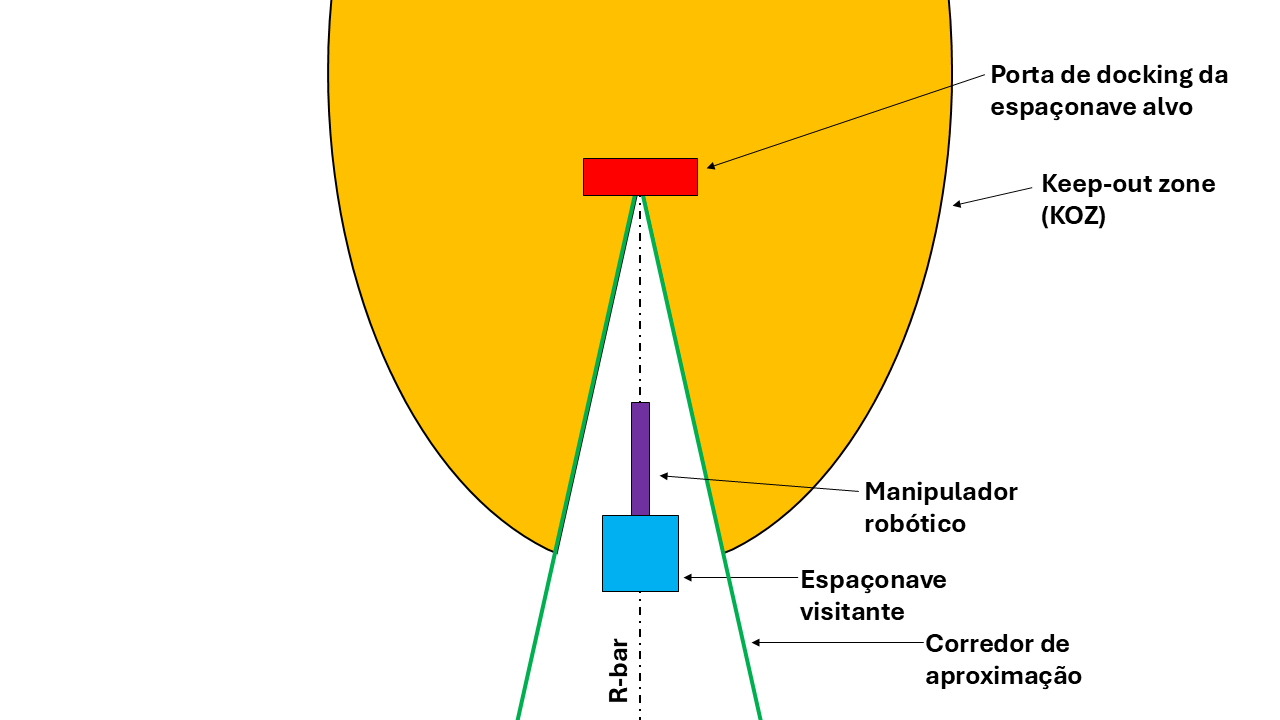
\includegraphics[width=1\linewidth]{3 Estrategia de RVDB/Imagens/2 Corredor e KOZ.png}
\caption{Corredor de aproximação e Keep-out zone.}
\end{figure}

\subsection{Corredor de aproximação}

Considerando o referencial LVLH do alvo, sendo seu eixo $x$ alinhado longitudinalmente no eixo radial (R-bar), $y$ alinhado com o vetor velocidade (\emph{along-track}) orbital e $z$ no eixo normal ao plano orbital.
O visitante deve permanecer em todo o tempo dentro do corredor de aproximação.

\subsection{Zona de exclusão}

A \emph{Keep-out Zone} (KOZ) de formato elipsoidal em torno da porta de acoplamento é utilizada como uma região proíbida onde o visitante não pode estar pois interfere na segurança da missão. Nessa região existe o risco do visitante colidir com outras partes físicas da espaçonave alvo.

\subsection{Infração da KOZ}

Caso o visitante entre na zona de exclusão, a aproximação final (ou curta) será abortada e o veículo deverá retornar ao ponto de espera anterior e realizar novas checagens.



% \subsection{Perfil de atitude e alinhamento de eixos}
\label{sec:perfil_atitude}

Durante as fases de injeção, faseamento e transferências orbitais, o controle de atitude é mantido em relação ao referencial inercial (ECI).
Sendo assim, o vetor de empuxo principal é orientado conforme o plano orbital da manobra, e o sensor de atitude absoluto (IMU) assegura o apontamento adequado do eixo de propulsão.
Nas fases de aproximação longa e final, o controle é definido no referencial LVLH do alvo.
O visitante alinha seu eixo longitudinal ao eixo radial da porta de acoplamento, de modo que o vetor de aproximação coincida com o eixo ${x}$ do referencial do alvo.
O eixo transversal ${y}$ é ajustado paralelamente ao eixo da velocidade orbital, e por fim, o eixo normal ${z}$ é mantido perpendicular ao plano da órbita.

O alinhamento é realizado de forma progressiva conforme a distância diminui.
Inicialmente, o visitante adota uma orientação na qual a atitude é estabilizada em relação ao ECI. Em seguida, o sistema de controle utiliza medidas relativas de atitude, obtidas pelo sensor LIDAR, para orientar a espaçonave em direção à porta de acoplamento.

Durante a fase de aproximação curta, a orientação é refinada para que o eixo de acoplamento do visitante coincida com o do alvo, dentro de uma tolerância angular reduzida.
O MR é posicionado de modo que sua ferramenta de acoplamento se estenda ao longo do eixo radial para acoplar a ferramenta na interface mecânica.
% \section{Integração com guiagem e controle}
\label{sec:integracao_guiagem_controle}

\subsection{Integração dos módulos de GNC}

A arquitetura de guiagem, navegação e controle é composta por três módulos principais:

\begin{enumerate}[label=(\roman*), leftmargin=*, itemsep=0pt]
    \item \textbf{Guiagem}: responsável pela trajetória nominal e pela geração de referências de posição e velocidade para cada fase da missão. Inclui as manobras orbitais de faseamento e as transferências de Hohmann, executadas no referencial inercial (ECI).
    \item \textbf{Navegação}: estima o estado do veículo visitante a partir dos sensores disponíveis.
    \item \textbf{Controle}: executa as leis de controle, ajustando as forças e torques exercidos para seguir as referências fornecidas pelo módulo de guiagem.
\end{enumerate}

\subsection{Comutação entre controladores}

Durante o processo de aproximação, ocorre a comutação entre diferentes modos de controle de acordo a distância ao alvo.
A lógica de comutação é ativada quando a distância relativa e a velocidade residual atingem limites pré-definidos.
A transição é feita de forma suave e automática, permitindo estabilidade e continuidade nas variáveis de estado e evitando descontinuidades numéricas.

\subsection{Adaptação de ganhos}

Os ganhos do controlador PD são ajustados conforme o regime operacional.
Em grandes distâncias, prevalece o termo proporcional, para reduzir o erro  de posição.
Conforme o visitante se aproxima do alvo, o termo derivativo possuir maior influência, pois aumenta a rigidez do sistema e amortece as oscilações de velocidade relativa.

\subsection{Arquitetura funcional do controle}

A arquitetura de controle foi estabelecida da seguinte forma:

\begin{enumerate}[label=(\roman*), leftmargin=*, itemsep=0pt]
    \item o módulo de guiagem fornece as trajetórias e as referências orbitais;
    \item o módulo de navegação recebe o estado do visitante e calcula as variáveis relativas;
    \item o módulo de controle executa as leis de comando, com ganhos adaptativos conforme o regime.
\end{enumerate}
% \section{Critérios de sucesso}
\label{sec:criterios_sucesso}

Os critérios de sucesso estabelecem as condições mínimas que definem o êxito da operação de RVD/B.

\subsection{Primários}

\begin{enumerate}[label=(\roman*), leftmargin=*, itemsep=0pt]
\item \textbf{Conclusão do acoplamento:} o visitante deve concluir o acoplamento dentro da janela temporal definida para a operação.

\item \textbf{Sem violação de segurança:} a trajetória da aproximação curta deve respeitar integralmente as zonas de segurança estabelecidas, conforme:
    \begin{enumerate}[label=(\alph*), itemsep=0pt]
    \item nenhuma entrada na \textit{keep-out zone} (KOZ);  
    \item permanência contínua dentro do corredor de aproximação durante toda a aproximação curta.
    \end{enumerate}

\item \textbf{Taxa de aproximação no contato:} a velocidade relativa entre o visitante e o alvo no momento de contato deve permanecer abaixo do limite máximo estabelecido para o acoplamento.

\item \textbf{Alinhamento no acoplamento:} o visitante deve atingir o contato mantendo a orientação e o posicionamento dentro dos limites de alinhamento especificados, conforme:
    \begin{enumerate}[label=(\alph*), itemsep=0pt]
    \item erro relativo de orientação dentro da margem aceitável;  
    \item desalinhamento lateral inferior aos limites definidos para a interface mecânica.
    \end{enumerate}
\end{enumerate}

\subsection{Desempenho de guiagem e controle}

Avaliou-se os erros relativos de posição, velocidade e atitude e a coerência das comutações entre modos.

\begin{enumerate}[label=(\roman*), leftmargin=*, itemsep=0pt]
\item \textbf{Erro de posição e velocidade relativa:} analisado por fase, considerando as métricas de valor médio, quadrático médio (RMS) e valor máximo registrado durante cada regime de aproximação.

\item \textbf{Erro de atitude relativa e taxa angular:} a atitude do visitante em relação ao alvo deve manter-se estável durante a aproximação curta e final, com variações angulares dentro das margens pré-determinadas para o alinhamento.

\item \textbf{Número de comutações de modo:} as transições entre os diferentes ganhos do controlador PD e modos de guiagem devem ocorrer conforme a lógica definida, sem oscilações indesejadas ou comutação excessiva.
\end{enumerate}

\subsection{Recursos}

Os critérios aqui apresentados avaliam a eficiência do sistema quanto ao consumo de propelente e ao tempo de execução das manobras.

\begin{enumerate}[label=(\roman*), leftmargin=*, itemsep=0pt]
\item \textbf{$\Delta v$ total:} é a soma de todos os incrementos de velocidade aplicados durante as fases de transferência e aproximação.

\item \textbf{Margem de propelente remanescente:} representa a diferença entre o propelente disponível após o acoplamento e a quantidade inicial de propelente.
\end{enumerate}

\subsection{Conformidade operacional e segurança}

Os critérios de conformidade operacional e segurança avaliam se a missão foi conduzida dentro dos limites definidos para cada fase da aproximação.

\begin{enumerate}[label=(\roman*), leftmargin=*, itemsep=0pt]
\item \textbf{Violações de limites por fase:} devem ser analisadas separadamente para:
    \begin{enumerate}[label=(\alph*), itemsep=0pt]
    \item velocidade relativa;  
    \item atitude;  
    \item saída do corredor de aproximação.
    \end{enumerate}

\item \textbf{Registro de violações:} cada evento deve ser documentado quanto à quantidade e à duração, sendo que ambos os indicadores devem ser nulos para que a manobra seja considerada aprovada.
\end{enumerate}

\subsection{Manipulador robótico}

Devido à arquitetura 4R1P adotada, o desempenho do manipulador robótico é avaliado em respeito ao acoplamento, para que seja realizado de forma precisa, sem esforços excessivos sobre a interface mecânica.

\begin{enumerate}[label=(\roman*), leftmargin=*, itemsep=0pt]
\item \textbf{Posicionamento da ferramenta:} o erro de pose da ferramenta na fase de pré-captura deve permanecer dentro da margem de tolerância definida, cuidando o alinhamento entre a junta prismática e a porta de acoplamento.

\item \textbf{Força e torque de contato:} durante o engate, as forças e torques aplicados pela ferramenta devem permanecer dentro dos limites operacionais especificados para a interface.

\item \textbf{Tempo de estabilização pós-contato:} logo após o engate, o acoplamento entre base--manipulador deve ser estável dentro do tempo previsto e sem oscilações perceptíveis.
\end{enumerate}

% \section{Parâmetros pré-definidos}

Nesta seção serão apresentados todos os parâmetros pré-definidos para todas as fases da missão.
Esses parâmetros são os dados de entrada para as simulações computacionais na plataforma MATLAB e Simulink.



